%
% teil3.tex -- Beispiel-File für Teil 3
%
% (c) 2020 Prof Dr Andreas Müller, Hochschule Rapperswil
%
% !TEX root = ../../buch.tex
% !TEX encoding = UTF-8
%
\subsection{Selektion
\label{buch:paper:varalg:subsection:selection}}
\rhead{Selektion}
In diesem Schritt werden Elternpaare ausgesucht, die später 
neue Nachkommen erzeugen. Die Selektion erfolgt so, dass in der 
Regel nur die Fittesten neue Kinder erzeugen.
Die Idee dahinter ist, dass es verschiedene Individuen gibt, 
die unterschiedlich fit sind. Die fitteren Individuen paaren 
sich eher, während die schwächeren seltener Nachwuchs erzeugen. 
So ähnlich wie in der Natur. Die Paare werden im System zufällig 
gewählt, aber die Wahrscheinlichkeit, dass die fitteren 
Individuen Nachkommen zeugen, ist höher.

\begin{figure}
    \centering
    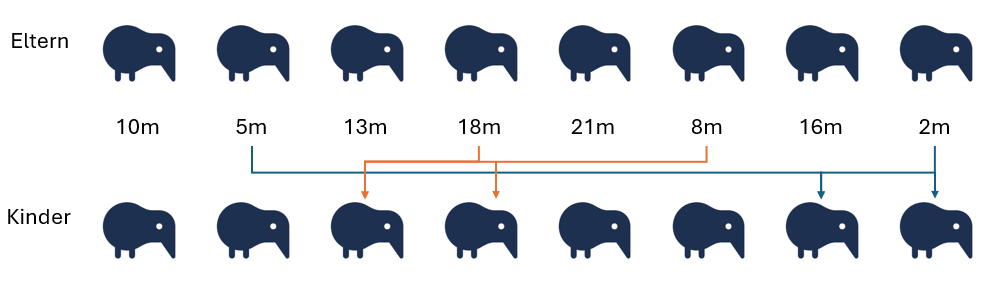
\includegraphics[width=0.8\textwidth]{
        papers/varalg/images/teil3/04OffspringProbability.png
    }
    \caption{Mögliche ausgewählte Eltern für Nachkommen}
    \label{fig:selection_of_parents}
\end{figure}
%TODO besser beschreiben wass gemeint ist
Auf dem Bild \ref{fig:selection_of_parents} sind Eltern mit unterschiedlichen
Weglänge. Dabei ist die Wahrscheinlichkeiten, dass sich die blaue Linie ereignet 
viel grösser als die Rote Linie. Diese ist aber trotzdem möglich.
\\
Für die Selektion gibt es verschiedene Möglichkeiten.
\\
1. **Roulette-Rad-Selektion:** 
- Individuen werden zufällig und proportional zu ihrer 
Fitness ausgewählt. Die Wahrscheinlichkeit wird anhand ihrer 
Fitness definiert. Kürzere Strecken haben eine höhere Chance, 
ausgewählt zu werden. Die Wahrscheinlichkeit wird mit einer 
entsprechenden Formel berechnet.

\begin{equation}
    \label{eq:probability_fittest}
    P_i = \frac{f_i}{\sum_{j=1}^{N} f_j}
\end{equation}

2. **Rangselektion:**
- Individuen werden nach ihrer Fitness sortiert und basierend 
auf ihrem Rang ausgewählt. Die Wahrscheinlichkeit wird anhand 
des Rangs definiert.

\begin{equation}
    \label{eq:probability_rating}
    P_i = \frac{r_i}{\sum_{j=1}^{N} r_j}
\end{equation}

3. **Turnierselektion:**
- Eine Gruppe von Individuen wird zufällig ausgewählt, und 
das fitteste Individuum dieser Gruppe wird als Elternteil gewählt.

Es gibt auch die Möglichkeit, ein eigenes Selektionssystem zu entwickeln, 
das ein Ausscheidungsverfahren beinhaltet, aus dem schließlich ein 
Elternpaar hervorgeht. Das System folgt einem logischen Ablauf, wobei 
die Wahrscheinlichkeit mathematisch berechnet wird.

\subsection{Selektion auf das TSP umgesetzt
\label{buch:paper:varalg:subsection:selection_tsp}}
\rhead{Selektion TSP}